\documentclass[11pt]{article}
\usepackage[margin = 1in]{geometry}
\usepackage{amsmath}
\usepackage{amssymb}
\usepackage{amsthm}
\usepackage{graphicx}
\usepackage{subfig}
\usepackage{enumitem}
\usepackage{url}
\usepackage[parfill]{parskip}
\newcommand{\skipline}{\vspace{\baselineskip}}
\newenvironment{problem}[1]{\textbf{Problem #1: }}{\newpage}


\begin{document}
	
	\begin{center}
		\textbf{Assignment 1} \\
		\textbf{Intro Math Modeling} \\
		\textbf{Math 336} \\
		\textbf{Stephen Giang RedID: 823184070} \\
	\end{center}

	\begin{problem}{1 (Exercise 1.1)}
		Two bodies with masses equal to $m_1$ and $m_2$. The distance between their centers of mass is $r$. The law of universal gravitation states that the two bodies attract each other with an attraction force equal to
		\[F_g = G \frac{m_1m_2}{r^2} \tag{1.77}\]
		Find the dimension of the universal gravitational constant $G$.
		\\ \\
		Notice that the dimension of force, ${[F]} = MLT^{-2}$.  Notice that we can take the dimension of the following:
		\[\frac{m_1m_2}{r^2} = \frac{M^2}{L^{2}} = M^2L^{-2}\]
		So now we can see the following:
		\begin{align*}
			[F] &= MLT^{-2} = [G]\,M^2L^{-2} \\
			[G] &= M^{-1}L^{3}T^{-2}
		\end{align*}
	\end{problem}

	\begin{problem}{2 (Exercise 1.6)}
		\begin{enumerate}[label = (\alph*)]
			\item Draw at least two diagrams to illustrate the nuclear shock wave problem in Section 1.5 
			\begin{figure}[h!]
				\centering
				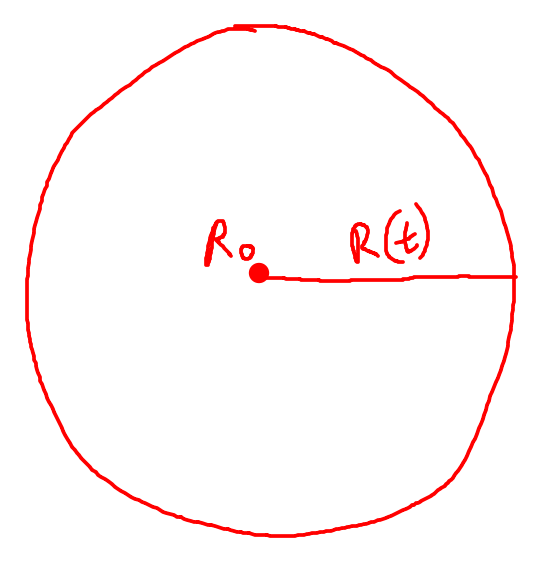
\includegraphics[width=6cm, height = 5cm]{Photos/RadiusShockWave.png}
				\hspace{1cm}
				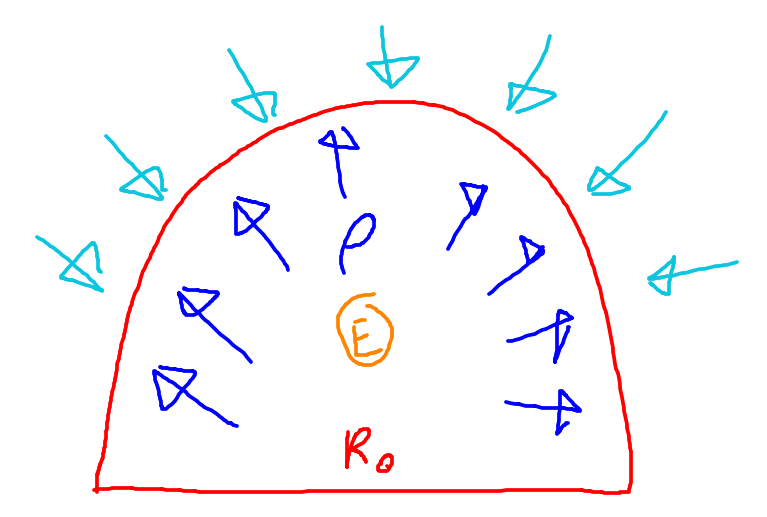
\includegraphics[width=8cm, height = 5cm]{Photos/Pressure.png}
			\end{figure}
			\item Write down the derivation details for the result equation: $R = \alpha \left(\frac{E}{\rho}\right)^{1/5}t^{2/5}$
			\\ \\
			Notice the dimension of the following equation:
			\begin{center}
				$R = \alpha E^{a}\rho^b t^c$ \\
				$=> [L] = 1 \times \left(ML^2T^{-2}\right)^a\left(ML^{-3}\right)^b T^c = M^{a+b}L^{2a-3b}T^{-2a+c}$
			\end{center}
			Now we get a simple system of equations:
			\begin{align*}
				a+b &= 0 \\
				2a-3b &= 1 \\
				-2a + c &= 0
			\end{align*}
			Solving this, we get that $a = \frac{1}{5}, b = \frac{-1}{5}, c = \frac{2}{5}$.  Thus we get the following:
			\[R = \alpha E^{1/5}\rho^{-1/5}t^{2/5} = \alpha \left(\frac{E}{\rho}\right)^{1/5}t^{2/5}\]
			\item Discuss the problem assumptions and the result.
			\\ \\
			We assume that the pressure caused by the nuclear explosion is much bigger than the atmospheric pressure, such that gravity is negligible.  We also assume that the only factors in determining the radius of the shock wave to be the amount of total energy, $E$, the pressure, $\rho$, and time, $t$.  Because of the powers of the factors dont equal 0, we know that these factors are necessary, and we know we have enough factors because the dimensional analysis leads to the desired result. Lastly, we get the result that the radius, $R$, is dependent on the fifth power of density times length, $Et^2$.
		\end{enumerate}
	\end{problem}
	
	\begin{problem}{3 (Exercise 1.7)}
		\begin{enumerate}[label = (\alph*)]
			\item Use dimensional analysis to find the period $\tau$ of the oscillation as a function of mass, spring constant $k$, gravitational acceleration $g$, for the mass-spring system shown in the figure below. The formula is determined up to a free dimensionless constant. 
			\\ \\
			Notice the following and let $\alpha$ be the dimensionless constant:
			\begin{center}
				$\tau = \alpha m^a k^b g^c$ \\
				$T = 1\times M^a (MT^{-2})^b (LT^{-2})^c = M^{a+b}L^cT^{-2b - 2c}$
			\end{center}
			Now we get a simple system of equations:
			\begin{align*}
			a+b &= 0 \\
			-2b-2c &= 1 \\
			c &= 0
			\end{align*}
			Solving this, we get that $a = \frac{1}{2}, b = \frac{-1}{2}, c = 0$.  Thus we get the following:
			\[\tau = \alpha m^{1/2}k^{-1/2} = \alpha \sqrt{\frac{m}{k}}\]
			\item Design an experiment to determine this constant. You do not have to actually do the experiment
			\begin{figure}[h!]
				\centering
				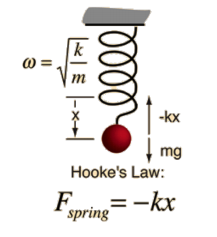
\includegraphics[]{Photos/HookesLaw.png}
			\end{figure}
			\\
			For the experiment, we can tie a spring to a mass, $m$, and drop the mass at an initial height and measure when it will come back up to its original height. That will determine our period, $\tau$.  We can find the spring constant by measuring the distance of the mass from its initial height to its lowest height, or the height when the spring starts to compress again. By measuring that distance, x, we get that the spring constant, $k = \frac{mg}{x}$, where $g$ is the acceleration of gravity. Then we get the following equation to solve for the constant, $\alpha$.
			\[\tau \sqrt{\frac{k}{m}} = \alpha\]  
		\end{enumerate}
	\end{problem}
	
	\begin{problem}{4}
		Derive the formula (1.54) on Page 11 for the speed of a free fall body from Eq. (1.40) at
		the beginning of Sub-section 1.4.4 on Page 10. You basically repeat what was done in the
		book, fill in the details not included in the book, and explain each of your steps. 
		\\ \\
		To do the dimensional analysis of the speed of a free fall body of mass, we assume that it depends on the following factors: mass, $m$, time, $t$, gravity, $g$, and distance, $h$.
		\\ \\
		\[v = \alpha m^a t^b g^c h^d\]
		So now we take its dimensions:
		\begin{center}
			$[v] = \alpha [m]^a[t]^b[g]^c[h]^d$ \\
			\vspace{.2cm}
			$LT^{-1} = 1 \times M^a T^b (LT^{-2})^c L^d = M^a T^{b-2c}L^{c+d}$
		\end{center} 
		Now we get a simple system of equations:
		\begin{align*}
			a &= 0 \\
			b - 2c &= -1 \\
			c + d &= 1
		\end{align*}
		Because we have a system of 4 variables, we can assume that one of the variable is redundant in the sense that we can drop on of the variables.  If we drop the variable $h$, and assume its dependent on time, we can make $d = 0$.  Thus we get that $c = 1, b = 1$.  This will then lead to the following:
		\[v = \alpha gt \]
		However, if we drop the time variable, $t$, and make $b = 0$, we get $c = d = \frac{1}{2}$, such that:
		\[v = \alpha\sqrt{gh}\] 
		Notice we can find $\alpha$ using the equality relating the conversion of potential energy into kinetic energy.
		\begin{align*}
			E_P = mgh = \frac{1}{2}mv^2 &= E_K \\
			mgh = \frac{1}{2}m(\alpha \sqrt{gh})^2 &= \frac{1}{2}\alpha^2 mgh \\
			1 &= \frac{1}{2}\alpha^2 \\
			\sqrt{2} &= \alpha 
		\end{align*}  
		Thus we get the following result:
		\[v = \sqrt{2gh}\]
	\end{problem}

	\begin{problem}{5}
		Exercise 1.13: The question is to find the period $\tau$ of the harmonic oscillation
		using an assumed model. The problem is already solved. What you need to do is
		to fill in more details and present a complete solution in your own way. 
		\\ \\
		We can use a simple harmonic sine function to model a pendulums position:
		\[\theta = A\sin(\omega t + B)\]
		with $A$ being the oscillation amplitude, $B$ is the phase, and $\omega$ is the circular frequency. 
		Suppose we release the pendulum at $t = 0$ and it reaches its highest points at $\theta = A$, then $B = \frac{\pi}{2}$ because $\sin\left(\frac{\pi}{2}\right)= 1$.  The period of $\sin x$ is $2\pi$, which is dimensionless.  Our pendulum's period is $\tau$, with its dimension being $T$. We know that the coefficient to $t$, inside a sine transformation, is always equal to the original period, $2\pi$ divided by the actual period, $\tau$.  So we get the following:
		\[\omega = \frac{2\pi}{\tau}\]
		Now we get the following equation:
		\[\theta = A\sin\left(\frac{2\pi t}{\tau} + \frac{\pi}{2}\right)\]
		Notice we can find the height, $h$, using the following model:
		\begin{figure}[h!]
			\centering
			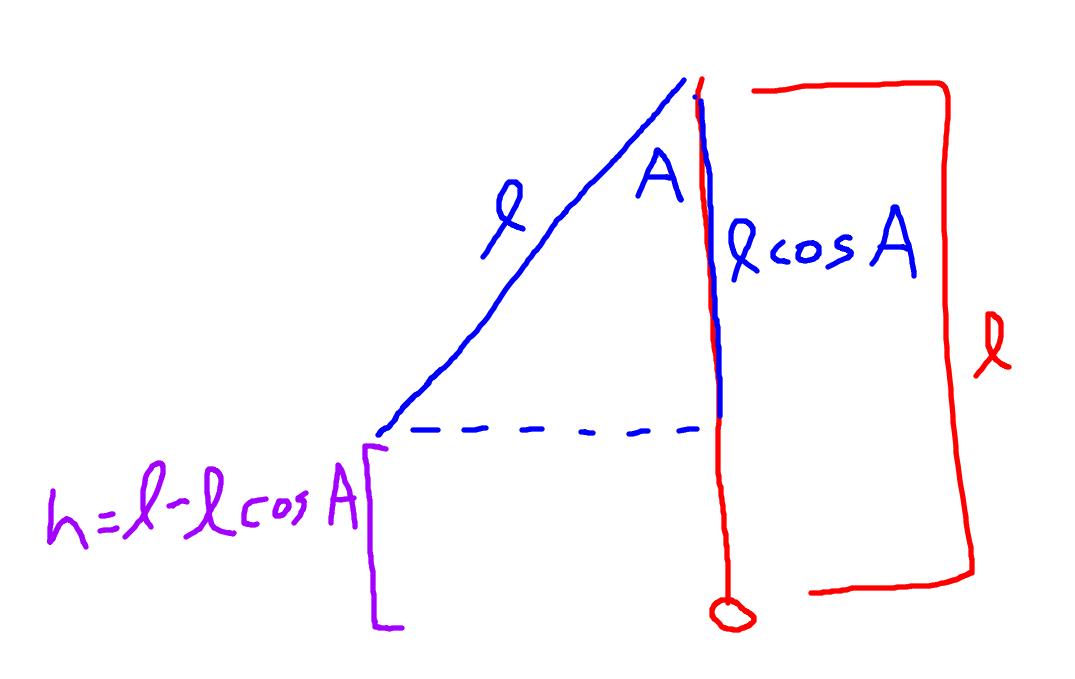
\includegraphics[width = 8cm]{Photos/Pendulum.png}
		\end{figure}
		\\
		At the highest point of the pendulum mass, the height, $h$, relative to the reference point of the potential energy is the following with $l$, being the length of pendulum:
		\[h = l - l\cos(A) = l(1 - \cos(A)) = 2l\sin^2\left(\frac{A}{2}\right)\]
		Now we can find the pendulums velocity, as it is the derivative of its position function multiplied by the length of the pendulum, as velocity depends on the length:
		\[v = l\frac{d\theta}{dt} = \frac{2lA\pi}{\tau}\cos\left(\frac{2\pi t}{\tau} + \frac{\pi}{2}\right)\]
		The pendulum reaches its maximum speed at its lowest point when $\cos\left(\frac{2\pi t}{\tau} + \frac{\pi}{2}\right) = 1$, so we get:
		\[v_{max} = \frac{2lA\pi}{\tau}\]
		Now we know that the potential energy, $E_P = mgh$ at the highest point is equal to the kinetic energy, $E_K = \frac{1}{2}mv^2$ at the lowest point:
		\[E_P = mg\left[2l\sin^2\left(\frac{A}{2}\right)\right] = \frac{1}{2}m\left[\frac{2lA\pi}{\tau}\right]^2 = E_K\]
		Notice we can linearize our sine function to get the following:
		\[\sin\left(\frac{A}{2}\right) = \frac{A}{2} - \frac{A^3}{2^3\,3!} + \frac{A^5}{2^5\,5!} + \cdots + (-1)^n \frac{A^{2n+1}}{2^{2n+1}\,(2n+1)!} \] 
		We can approximate this function now, for very small values of $A$, we can say that $\sin\left(\frac{A}{2}\right) = \frac{A}{2}$, such that we get the result:
		\[\sin^2\left(\frac{A}{2}\right) = \left(\frac{A}{2}\right)^2\]
		Now we can resubstitute this into our equation and get the following:
		\begin{align*}
			 mg\left[2l\left(\frac{A}{2}\right)^2\right] &= \frac{1}{2}m\left[\frac{2lA\pi}{\tau}\right]^2 \\
			 \frac{1}{2}mglA^2 &= 2ml^2A^2\pi^2\tau{-2} \\
			 \tau^2 &= \frac{4\pi^2 l}{g} \\
			 \tau &= 2\pi \sqrt{\frac{l}{g}}
		\end{align*}
		Finally we can resubstitute this in with $\omega = \frac{2\pi}{\tau} = \sqrt{\frac{g}{l}}$:
		\[\theta = A\sin\left(\sqrt{\frac{g}{l}} t + \frac{\pi}{2}\right)\]
	\end{problem}
		











\end{document}
